%% LyX 1.6.4 created this file.  For more info, see http://www.lyx.org/.
%% Do not edit unless you really know what you are doing.
\documentclass[oneside,english,final]{amsart}
\usepackage[T1]{fontenc}
\usepackage[latin9]{inputenc}
\usepackage{textcomp}
\usepackage{amsthm}
\usepackage{graphicx}

\makeatletter
%%%%%%%%%%%%%%%%%%%%%%%%%%%%%% Textclass specific LaTeX commands.
\numberwithin{equation}{section} %% Comment out for sequentially-numbered
\numberwithin{figure}{section} %% Comment out for sequentially-numbered

\makeatother

\usepackage{babel}

\begin{document}

\title{HiFlow\textthreesuperior{} - The Flexible Lib }

\maketitle

\section{Module DoF / FEM}

In context of the finite element method (FEM), the existing degrees
of freedom (DoFs) of a discrete function must be numbered. The treatment
of local numbering (within a given reference cell) and the corresponding
global numbering (within the given mesh) respresents a non-trivial
task, especially with respect to performance and generality. In the
following the interface approach of HiFlow\textthreesuperior{} is
discribed.


\subsection{Problem definition}

Given an unstructured mesh consisting of various cell types, e.g.
triangles, quadrilaterals, hexahedrons, tetrahedrons, there is the
task to create some unique numbering of the existing degrees of freedom
on the global mesh. Given some local numbering procedure for each
cell the correspondence between locally unique DoFs on a given cell
and globally unique DoF Ids must be calculated. For many applications
some constraints for DoFs of neighbouring cells exist. For example
the approximation of continuous functions requires interpolation or
identification of some local DoFs by DoFs of the neighbouring cells.
These constraints must be determined and managed which is challenging
not only in the case of adaptive methods (h-, p- or hp-refinement)
but also in the non - adaptive case regarding performance (consider
for expample the numbering of some huge three dimensional geometry
containing a lot of cells). In figure \ref{fig:Degrees-of-freedom}
the DoFs of an hp-refined discretization are visualized by the dots,
where green dots represent constrained DoFs in case of a global continuity
condition.

%
\begin{figure}
\noindent \begin{centering}
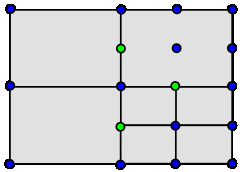
\includegraphics[height=3cm]{images/dof1}
\par\end{centering}

\caption{\label{fig:Degrees-of-freedom}Degrees of freedom in hp-refined setting.}

\end{figure}



\subsection{Solution procedure}

For each finite element ansatz the number and the geometric location
of the degrees of freedom are defined on the corresponding reference
cell only. The local numeration of the DoFs is defined at one specific
place and is chosen to be a lexicographic numeration systematically.
The DoFs in any cell of the considered mesh are determined by a transformation
that maps the reference cell to the chosen physical cell and thereby
defines the location of the DoF points (see figure \ref{fig:Transforming-DoF-points}).
At that state the DoF Ids can be defined and are numbered consecutively
in the order of a given iteration through the mesh cells and the local
numeration scheme. Further a mapping that maps a cell index of the
mesh and a local DoF index (key) to the corresponding DoF Id (value)
is created.

For the calculation of the interpolation and identification of DoFs
on neighbouring cells an interface approach is realized, where in
this context \emph{interface} denotes the common cell boundary between
two neighbouring cells. Through an iteration over all such interfaces,
a so-called \emph{interface pattern} is determined that includes the
geometrical information (orientation of cells, h-refinement status,
etc.) as well as the finite element ansatz of the participating cells
such that all information needed to characterize the interface is
included. With the information contained in the pattern the corresponding
DoF interpolation and identification in terms of the local DoFs are
calculated. Therefore the general transfer operator of Schieweck \cite{Schieweck}
is used that allows for interpolation between different finite element
spaces. An important step within this phase is the transformation
of DoFs of a neighbouring cell next to the reference cell (see figure
\ref{fig:Transforming-DoF-points}). Once this local evaluation is
done, the tuple of the pattern description (key) and the interpolation
and identification information (value) are stored in a map structure
that allows for fast access given a pattern description. Using this
map the interpolation and identification of DoF Ids can be realized
efficiently even in the complex hp-refined context using the equivalence
class generator in \cite{Crecipes}. Lateron the numbering of the
DoF Ids can be changed easily by applying some user defined permutation.

%
\begin{figure}
\noindent \begin{centering}
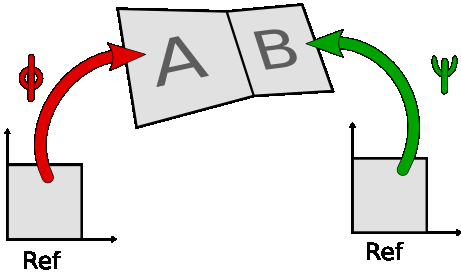
\includegraphics[height=3cm]{images/dof3}\hfill{}\hfill{}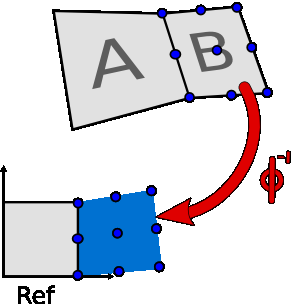
\includegraphics[height=3cm]{images/dof5}
\par\end{centering}

\caption{\label{fig:Transforming-DoF-points}Transforming DoF points to cell
in mesh (left). Transformation of DoFs of neighbouring cell next to
the reference cell (right).}

\end{figure}



\subsection{Parallelization issues}

In a domain decomposition setup, i.e. several processes are used for
the solution of one single domain, each part of the domain (subdomain)
is dedicated to one process using MPI. Again a unique DoF numeration
of all DoFs in the global domain must be determined. For good scaling
properties, a parallel and distributed handling of the DoFs is needed,
i.e. each process manages the DoFs that are connected to the cells
lying in its domain and a \emph{DoF partitioner} is used to create
the correspondence with other subdomains from other processors via
MPI communication. Each subdomain has information of the neighbouring
domains by the \emph{ghost cells} (one \emph{ghost layer}), which
are represented by the red cells in figure \ref{fig:Two-domains-with}.
To create a DoF numering with (domain-) global Ids, each process determines
in a first step a consecutive numering of the DoFs within its subdomain,
whereas also the ghost layer is treated as if it would belong to the
subdomain. Next, the wrong information stored in this layer needs
to be updated via communication. Hereby, a decision needs to be made,
wheter a DoF lying on the sceleton of the domain belongs to a subdomain
or not, i. e. this DoF is lying on two subdomains, which are sharing
it. The implemented procedure states, that the subdomain represented
by a unique lower subdomain Id will own the DoF. Hence, the idenification
and interpolation procedure can be established. At the final stage,
every subdomain has a unique numbering, containing the correct DoF
Ids in the ghost layer.
\begin{itemize}
\item %
\begin{figure}
\begin{centering}
\includegraphics[height=4cm]{images/dof6}
\par\end{centering}

\caption{\label{fig:Two-domains-with}Two domains with ghost cells}



\end{figure}
\end{itemize}
\begin{thebibliography}{2}
\bibitem{Schieweck} Schieweck, F. A General Transfer Operator for
Arbitrary Finite Element Spaces. Techreport, University Magdeburg,
2000.

\bibitem{Crecipes} W. Press, S. Teukolsky, W. Vetterling, B. P. Flannery,
\textquotedbl{}Numerical Recipes in C\textquotedbl{}, Second edition,
Cambridge University Press, pages 345 / 346
\end{thebibliography}

\end{document}
